% Options for packages loaded elsewhere
\PassOptionsToPackage{unicode}{hyperref}
\PassOptionsToPackage{hyphens}{url}
\PassOptionsToPackage{dvipsnames,svgnames,x11names}{xcolor}
\documentclass[
  10pt,
  fontset=fandol]{ctexart}
\usepackage{xcolor}
\usepackage[margin=16mm]{geometry}
\usepackage{amsmath,amssymb}
\setcounter{secnumdepth}{-\maxdimen} % remove section numbering
\usepackage{iftex}
\ifPDFTeX
  \usepackage[T1]{fontenc}
  \usepackage[utf8]{inputenc}
  \usepackage{textcomp} % provide euro and other symbols
\else % if luatex or xetex
  \usepackage{unicode-math} % this also loads fontspec
  \defaultfontfeatures{Scale=MatchLowercase}
  \defaultfontfeatures[\rmfamily]{Ligatures=TeX,Scale=1}
\fi
\usepackage{lmodern}
\ifPDFTeX\else
  % xetex/luatex font selection
\fi
% Use upquote if available, for straight quotes in verbatim environments
\IfFileExists{upquote.sty}{\usepackage{upquote}}{}
\IfFileExists{microtype.sty}{% use microtype if available
  \usepackage[]{microtype}
  \UseMicrotypeSet[protrusion]{basicmath} % disable protrusion for tt fonts
}{}
\makeatletter
\@ifundefined{KOMAClassName}{% if non-KOMA class
  \IfFileExists{parskip.sty}{%
    \usepackage{parskip}
  }{% else
    \setlength{\parindent}{0pt}
    \setlength{\parskip}{6pt plus 2pt minus 1pt}}
}{% if KOMA class
  \KOMAoptions{parskip=half}}
\makeatother
\usepackage{longtable,booktabs,array}
\newcounter{none} % for unnumbered tables
\usepackage{calc} % for calculating minipage widths
% Correct order of tables after \paragraph or \subparagraph
\usepackage{etoolbox}
\makeatletter
\patchcmd\longtable{\par}{\if@noskipsec\mbox{}\fi\par}{}{}
\makeatother
% Allow footnotes in longtable head/foot
\IfFileExists{footnotehyper.sty}{\usepackage{footnotehyper}}{\usepackage{footnote}}
\makesavenoteenv{longtable}
\usepackage{graphicx}
\makeatletter
\newsavebox\pandoc@box
\newcommand*\pandocbounded[1]{% scales image to fit in text height/width
  \sbox\pandoc@box{#1}%
  \Gscale@div\@tempa{\textheight}{\dimexpr\ht\pandoc@box+\dp\pandoc@box\relax}%
  \Gscale@div\@tempb{\linewidth}{\wd\pandoc@box}%
  \ifdim\@tempb\p@<\@tempa\p@\let\@tempa\@tempb\fi% select the smaller of both
  \ifdim\@tempa\p@<\p@\scalebox{\@tempa}{\usebox\pandoc@box}%
  \else\usebox{\pandoc@box}%
  \fi%
}
% Set default figure placement to htbp
\def\fps@figure{htbp}
\makeatother
\setlength{\emergencystretch}{3em} % prevent overfull lines
\providecommand{\tightlist}{%
  \setlength{\itemsep}{0pt}\setlength{\parskip}{0pt}}
\usepackage{amsmath,amssymb,mathtools,needspace}
\xeCJKDeclareCharClass{CJK}{"2032,"0400->"04FF,"2160->"216B,"2460->"2473,"25A0,"25C7,"25CB,"25CF}
\IfFontExistsTF{Arial Unicode MS}{\xeCJKsetup{AutoFallBack=true}\setCJKfallbackfamilyfont{\CJKrmdefault}{Arial Unicode MS}}{}
\setcounter{secnumdepth}{0}
\setlength{\emergencystretch}{2em}
\allowdisplaybreaks
\usepackage{bookmark}
\IfFileExists{xurl.sty}{\usepackage{xurl}}{} % add URL line breaks if available
\urlstyle{same}
\hypersetup{
  pdftitle={数列求和的二分法},
  colorlinks=true,
  linkcolor={Maroon},
  filecolor={Maroon},
  citecolor={Blue},
  urlcolor={Blue},
  pdfcreator={LaTeX via pandoc}}

\title{数列求和的二分法}
\author{}
\date{}

\begin{document}
\maketitle

\subsubsection{11.2.3　数列求和的二分法}\label{ux6570ux5217ux6c42ux548cux7684ux4e8cux5206ux6cd5}

再考察所给和式（10.2.1），容易看出，如果将其奇偶项两两合并，即可使其规模变成 \(N_1=N/2\)，即

\[
S=\sum_{i=0}^{N_1-1}(a_{2i}+a_{2i+1})=\sum_{i=0}^{N_1-1}a_i^{(1)}.
\]

为此，所要施行的运算手续是

\[
a_i^{(1)}=a_{2i}+a_{2i+1},\quad i=0,1,\cdots,N_1-1.
\]

注意到这样加工出的求和问题

\[
S=\sum_{i=0}^{N_1-1}a_i^{(1)}
\]

与所给问题（10.2.1）属于同一类型，所不同的只是规模缩减了一半，因此上述加工手续是一种二分手续。

反复施行这种二分手续，二分 \(k\) 次后和式的项数压缩成 \(N_k=N/2^k\)，即

\[
S=\sum_{i=0}^{N_k-1}a_i^{(k)},
\]

式中

\[
a_i^{(k)}=a_{2i}^{(k-1)}+a_{2i+1}^{(k-1)},\quad i=0,1,\cdots,N_k-1.
\tag{11.2.4}
\]

这样二分 \(n=\log_2 N\) 次后，所给和式最终退化为一项，从而直接得出所求的和值 \(S\)。于是有数列求和的二分算法 11.2。

\textbf{算法 11.2}　对 \(k=1,2,\cdots\) 直到 \(n=\log_2 N\) 执行算式（11.2.4），结果有

\[
S=a_0^{(n)}.
\]

这一算法显然可以向量化。事实上，算式（11.2.4）可以表为向量形式：

\[
\begin{pmatrix}
a_0^{(k)}\\
a_1^{(k)}\\
\vdots\\
a_{N_k-1}^{(k)}
\end{pmatrix}
=
\begin{pmatrix}
a_0^{(k-1)}\\
a_2^{(k-1)}\\
\vdots\\
a_{N_{k-1}-2}^{(k-1)}
\end{pmatrix}
+
\begin{pmatrix}
a_1^{(k-1)}\\
a_3^{(k-1)}\\
\vdots\\
a_{N_{k-1}-1}^{(k-1)}
\end{pmatrix}.
\]

\begin{quote}
校注（agent 补充，CH11-E001）：本页两处回引均印作``（10.2.1）''，已照录；从本节的数列求和定义及上下文判断，应回引本章的式（11.2.1）。这是原书交叉引用疑误，不是 OCR 改写。
\end{quote}

\href{../../source-images/pdf-282.jpeg}{原页图像}

反复运用二分手续加工所考察的求和问题，逐步压缩和式的规模，最终加工成规模为 1 的最简形式，即可直接得出所求的解。由此可见，数列求和二分法的设计过程简洁而明快，如图 11.3 所示。

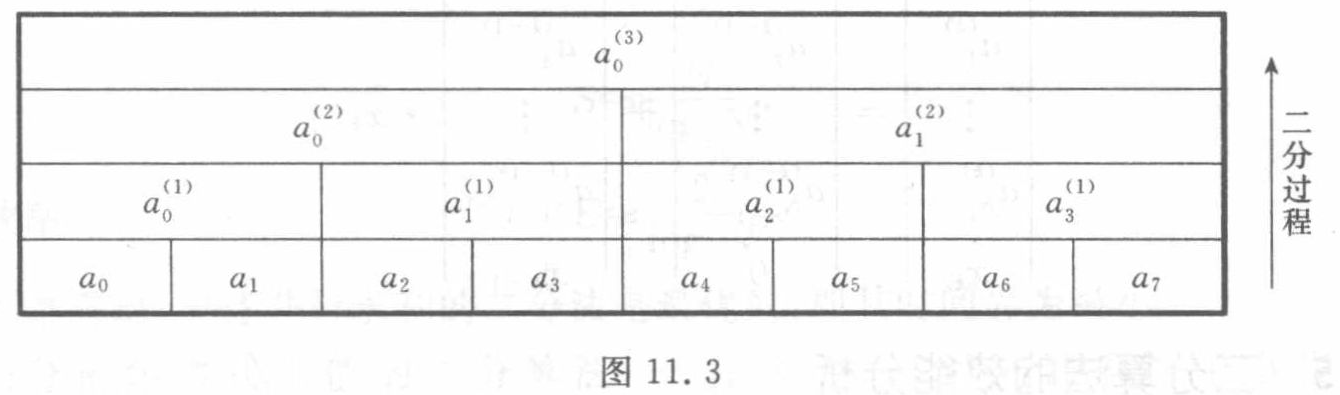
\includegraphics[width=0.85\linewidth,height=\textheight,keepaspectratio,alt={图 11.3（原图裁切）}]{../assets/ch11/figure-11-3.png}

图 11.3　原图``二分过程''箭头自下向上。各层从左至右的符号标签为：

{\def\LTcaptype{none} % do not increment counter
\begin{longtable}[]{@{}ll@{}}
\toprule\noalign{}
层次（由下至上） & 原图中的数据 \\
\midrule\noalign{}
\endhead
\bottomrule\noalign{}
\endlastfoot
初始层 & \(a_0\)，\(a_1\)，\(a_2\)，\(a_3\)，\(a_4\)，\(a_5\)，\(a_6\)，\(a_7\) \\
第 1 次二分 & \(a_0^{(1)}\)，\(a_1^{(1)}\)，\(a_2^{(1)}\)，\(a_3^{(1)}\) \\
第 2 次二分 & \(a_0^{(2)}\)，\(a_1^{(2)}\) \\
第 3 次二分 & \(a_0^{(3)}\) \\
\end{longtable}
}

每次将相邻两格合为上层的一格。（本段及上表为原图标签与结构的文字转录。）

应当指出的是，上面提供的两个算法------算法 11.1 和算法 11.2，尽管思路不同，繁简互异，但却是殊途同归。事实上，式（11.2.4）与式（11.2.3）得出的是同样的结果：

\[
a_i^{(k)}=S(2^ki+2^k-1,2^ki).
\]

\subsection{本节覆盖原页的校注记录}\label{ux672cux8282ux8986ux76d6ux539fux9875ux7684ux6821ux6ce8ux8bb0ux5f55}

下列记录按原页关联，含同页相邻小节的校注；计算时同时读取上文校注和完整原页。

\begin{itemize}
\tightlist
\item
  \texttt{CH11-E001}：原书 PDF 页 281
\end{itemize}

\end{document}
